\documentclass[authoryear, 1p]{elsarticle}
\usepackage[utf8]{inputenc}
\usepackage{caption} 
\usepackage{arydshln}
\captionsetup[table]{skip=5pt}
\usepackage{amsfonts,amssymb,graphics,epsfig,verbatim,bm,latexsym,amsmath,url,amsbsy}

\newtheorem{thm}{Theorem}
\numberwithin{equation}{section}

\begin{document}
\begin{frontmatter}
 
\title{GARCH-M model with an asymmetric risk premium: Distinguishing between 'good' and 'bad' volatility periods.} 

 \author[1]{Juri Trifonov\corref{cor1}}
\ead{jutrif98@gmail.com}
\author[2]{Bogdan Potanin} \ead{bogdanpotanin@gmail.com}

\cortext[cor1]{Corresponding author}

\affiliation[1]{organization={National Research University Higher School of Economics}, addressline={Pokrovsky Blvd 11},
postcode={109028}, city={Moscow}, country={Russia}}
\affiliation[2]{organization={National Research University Higher School of Economics}, addressline={Pokrovsky Blvd 11},
postcode={109028}, city={Moscow}, country={Russia}}


\begin{abstract}
We proposed the new method (GARCH-M-LEV) that allows capturing the asymmetry both in the variance and return equations. The development of the model is encouraged by the stylized fact that investors demand a higher risk premium during ''bad'' volatility periods rather than ''good'' ones. To study the properties of the obtained estimators, we conducted a simulated data analysis, considering a data generating process characterized by asymmetric responses of risk premium to volatility changes.
As a result, we have found statistical evidence in favor of a significant advantage of the proposed method compared to existing alternatives. Further, the proposed model was applied to study the S\&P 500 market index. During most periods under consideration, we have found evidence of an asymmetric relationship between the risk premium and volatility changes. Due to this reason, the GARCH-M-LEV model usually was able to outperform the alternative GARCH family models according to the information criterion.
\end{abstract}

\begin{keyword}
GARCH \sep leverage effect \sep risk premium \sep conditional volatility.
%% keywords here, in the form: keyword \sep keyword

%% PACS codes here, in the form: \PACS code \sep code

%% MSC codes here, in the form: \MSC code \sep code
%% or \MSC[2008] code \sep code (2000 is the default)
\JEL C18 \sep C22 \sep C58
\end{keyword}

\end{frontmatter}
\section*{Declaration of Interest}
\noindent The authors have no conflict of interests to declare.
\vspace{2pt}

\noindent \textit{This research did not receive any specific grant from funding agencies in the public, commercial, or not-for-profit sectors.}
\section*{CRediT author statement}
\begin{flushleft}
\textbf{Juri Trifonov:} development of the main idea, derivation of the unconditional variance, drafting the manuscript, and software implementation of the proposed method.

\textbf{Bogdan Potanin:} drafting the manuscript and software implementation of the proposed method.
\end{flushleft}


\newpage
\section{Introduction}\label{Section1}
Volatility is considered to be one of the most essential factors in financial markets. The indicator reflects assets' level of risk and usually is measured by the standard deviation of returns. Thus, volatility modelling is indispensable in risk management policy, option pricing models, and other fields of finance \citep{Miralles2013}. The GARCH family models, firstly introduced by \citep{Engle1982} and \citep{Bollerslev1986}, are supposed to be the most common method of modelling conditional volatility of financial assets. 

The introduction of GARCH encouraged the development of a new literature stratum dedicated to the creation of various GARCH type models. These modifications of classical GARCH were stimulated by the need of adapting the model to the financial theory and stylised facts that occur in financial markets.

According to the main portfolio theories of \citep{Markowitz1952} and \citep{Sharpe1964}, asset returns and volatility are the key factors that describe pricing. Specifically, returns and volatility have a positive correlation. Thus, investors demand higher returns when the asset is more volatile. This idea has become the foundation for the introduction of the main concept in financial economics. That is, the concept states that every risky asset incorporates a risk premium component in its return. Because classic GARCH models do not allow to account for a risk premium existence in the return equation, this led to the development of a new GARCH type model. The GARCH-in-Mean (GARCH-M) model has been introduced by \citep{Engle1987}. Its key feature was an incorporation of the conditional variance into the mean equation, introducing the contribution of the risk premium to the dynamics of returns. This model has become widely used by researchers. 
Nevertheless, \citep{Bollerslev2022} indicates that inconsistent results concerning the sign of the risk premium and its robustness have been found in several papers: \citep{Hong2020}, \citep{Rossi2015}, \citep{Bollerslev2006}. According to \citep{Bollerslev2022}, recent studies illustrate contradictory outcomes since the contribution sign of the risk premium differs among the periods and assets. Moreover, he suggests that such inconsistency may be caused by the asymmetric relation between volatility and return. The classic GARCH-M model does not allow to capture such asymmetry, thus, the estimator of the risk premium contribution may be inconsistent.

Although the concept of asymmetric relation is novel in the framework of the GARCH-M model, it has been extensively studied in the context of classic GARCH models and refers to the asymmetric responses of conditional variance to shocks in returns. There is a widely known stylised fact in financial markets that volatility reacts more sharply to negative shocks in returns rather than to positive ones \citep{Zhang2006} \citep{Black1976}. Because classical GARCH is symmetric, it does not allow to account for such effects \citep{Nelson1991}. This problem has led to the development of leveraged GARCH models that account for the asymmetry effect of random shocks in the variance equation. Most popular models of this type, including EGARCH \citep{Nelson1991} and GJR-GARCH \citep{Glosten1993}, have been focusing on the functional form of the asymmetry effect in the variance equation. Modern studies mainly concentrate on developing more flexible asymmetric specifications in variance equation \citep{PGARCH} or on the multivariate generalization of classical asymmetric GARCH models \citep{MGJR}. However, the concept of capturing asymmetric responses of returns to conditional volatility,  i.e. the asymmetry in the mean equation, is poorly studied in the literature. Our paper fills this gap by introducing the leverage effect in the mean part of the GARCH-M model.

In this study, we propose a new GARCH-M-GJR-LEV model that accounts for the asymmetry effect not only in the variance equation but also in the equation of returns. The model is constructed in the framework of GJR-GARCH and based on the idea that negative shocks in returns lead to the higher contribution of conditional volatilities to asset returns. In other words, the model includes an additional parameter in the mean equation that reflects the asymmetric response of returns to volatility changes.

According to the simulated data analysis results, we have found statistical evidence in favour of the significant advantage of the proposed method in comparison with other GARCH-type models. Moreover, using the log returns of the S\&P 500 index, we have found evidence in favour of an asymmetric risk premium existence over different time intervals.

The paper proceeds as follows: In the next section, we briefly introduce and discuss GARCH-M and GJR-GARCH specifications. Next, we introduce our model, explain the intuition and derive the unconditional variance of returns. In Section 4, we provide the results of the simulated data analysis. In Section 5, we apply our model to study the log returns of the S\&P500 index and discuss the results. Finally, we summarize our contribution and findings.

\section{The GARCH-M Model}\label{Section2}

Let's denote $y$ as a $T \times 1$ vector of log returns and $\sigma$ as a $T \times 1$ vector of conditional volatilities, where $T \in N$. Then without loss of generality, we can specify the GARCH-M(1,1) \citep{Engle1987} process with the following system of equations:
\begin{equation}
\begin{gathered}
y_{t} = \mu + \lambda \sigma_{t} + \varepsilon_{t}, \\ 
\sigma^2_{t} = \omega + \alpha \varepsilon^2_{t-1} + \beta \sigma^2_{t-1}, \\ 
\xi_{t} \sim \mathcal{N} \left(0,1\right) \; i.i.d., \\ 
\varepsilon_{t} = \sigma_{t} \xi_{t},  
\end{gathered}
\end{equation}
where parameters $\omega, \alpha,$ and $\beta$ determine the dynamics of conditional variance and $t\in\{1,\dots,T\}$. The distinctive feature of the model is the presence of $\sigma_{t}$ in the mean equation. Therefore, volatility is allowed to influence return directly, and, thus, $\lambda\sigma_{t}$ is usually interpreted as a risk premium. Based on the portfolio theories of \citep{Markowitz1952} and \citep{Sharpe1964}, $\lambda$ is expected to be positive because the increase in volatility leads to a higher return \citep{Engle1987}.

Although the model allows for capturing a risk premium effect, it may be easily seen that the specification does not allow to account for the asymmetric responses. In other words, returns react identically to changes in volatility without considering the sign of the shocks that caused it. Therefore, volatility during both ''bear'' and ''bull'' markets has the same effect on returns.

\section{The GJR-GARCH Model}\label{Section3}

The GJR-GARCH \citep{Glosten1993} model has been developed to capture the leverage effect in financial markets. We use the GJR-GARCH framework as the basis for our model since its theoretical properties are well studied even in the multivariate case \citep{MGJR}. The other possible alternative is EGARCH proposed by \citep{Nelson1991}. According to the empirical study of \citep{Awartani}, EGARCH has demonstrated the highest accuracy on S\&P 500 index data compared to various asymmetric GARCH-family models, including GJR-GARCH, TGARCH, and AGARCH. However, it is complicated to derive the theoretical properties of the EGARCH model since it is based on a complex random coefficient nonlinear moving average process whose stationarity conditions are still unknown \citep{EGARCH2014}. Moreover, according to \citep{Awartani}, GJR-GARCH performed as the second best (after EGARCH) when the author studied combinations of asymmetric GARCH models with a classical GARCH-M. Therefore we prefer GJR-GARCH over other asymmetric GARCH specifications as a starting point for our model because it is relatively easy to derive theoretical properties of its modifications (i.e. of GARCH-M-GJR-LEV), and it has demonstrated reasonably good performance on S\&P 500 index that we use in the empirical part of our study.

This process is identical to the classical GARCH specification but it allows for asymmetric responses of variance to shocks in returns. Following the notations from the previous model, the GJR-GARCH(1,1) process is specified as follows:
\begin{equation}
\begin{gathered}
y_{t} = \mu + \varepsilon_{t}, \\ 
\sigma^2_{t} = \omega + \alpha \varepsilon^2_{t-1} + \gamma I_{t-1} \varepsilon^2_{t-t} + \beta \sigma^2_{t-1}, \\ 
I_{t}=\begin{cases}0\text{, if }\varepsilon_{t}\geq 0 \\1\text{, if }\varepsilon_{t}< 0\end{cases},\\
\xi_{t} \sim \mathcal{N} \left(0,1\right) \; i.i.d., \\ 
\varepsilon_{t} = \sigma_{t} \xi_{t}.  
\end{gathered}
\end{equation}

The crucial feature of this model is that volatility may react differently to positive and negative shocks in returns. It is realized by including an indicator variable $I_{t}$ that reflects the sign of the shock in period $t$. Thus, it may be easily seen that in case the shock is positive, the contribution to volatility will be made only by the $\alpha$ parameter. In contrast, negative shocks will reflect a more sharp contribution to conditional volatility and will be equal to $\alpha + \gamma$.

It is straightforward to show that the unconditional mean and variance of the process are specified as:

\begin{equation}
\begin{gathered}
\mathbb{E} [y_{t}] = \mu, \\
Var \left(y_{t} \right) = \sigma^2 = \frac{1}{1 - \alpha - \gamma / 2 - \beta}.
\end{gathered}
\end{equation}
By definition, the unconditional variance should be positively defined. Therefore, we can easily impose the parameter constraints that ensure process stationarity:
\begin{equation}
\begin{gathered}
\omega > 0, \\
\alpha + \gamma/2 + \beta < 1.
\end{gathered}
\end{equation}

The model has been developed to account for the stylized fact about the asymmetric relationship between volatility and shocks in asset returns. According to \citep{Zhang2006} and \citep{Black1976}, there has been found statistical evidence that volatility reacts more sharply on negative shocks in returns rather than on positive ones. Therefore, the sign of $\gamma$ parameter, reflecting the leverage effect, is expected to be positive. The positive estimate will reflect more considerable volatility growth when the observed shocks are negative. There exist several approaches in the literature tending to explain the causes of the asymmetry effect. According to \citep{Black1976} and \citep{Christie1982}, negative shocks in return lead to an increase in the financial leverage of issuing companies. Consequently, higher leverage enlarges the stocks' level of risk and leads to an increase in their volatility. Moreover, according to the prospect theory of \citep{Kahneman1979}, the asymmetry effect can arise in the framework of investors' cognitive features. People tend to perceive losses more critically, and, therefore, negative shocks in return may result in massive asset sales among investors, thereby provoking an increase in volatility. 

\section{The GARCH-M-GJR-LEV Model} \label{Section4}

The classic GARCH-M model allows capturing risk premium in assets' returns. Albeit, the model does not allow for asymmetric responses of returns to risk premium fluctuations. Therefore, the process is not able to differentiate between signs of shocks that cause the volatility, i.e. it perceives negative and positive shocks equally. Thus, the GARCH-M imposes the assumption that investors demand similar risk premiums when the market experiences ''good'' and ''bad'' volatility periods. In other words, the model accounts only for the absolute value of shocks determining the risk premium.
Nevertheless, according to \citep{Bollerslev2022}, there has been found statistical evidence that GARCH-M may demonstrate insignificant risk premiums in asset returns. Moreover, some studies has shown that the model may provide negative estimates of a risk premium. Such results are inconsistent with the main portfolio theories of \citep{Markowitz1952} and
\citep{Sharpe1964} since they state an inverse risk-return relationship, implying a negative correlation between volatility and returns. Following \citep{Bollerslev2022}, the problem may be explained by the necessity of differentiation between ''good'' and ''bad'' volatility measures. Rational investors tend to demand a higher risk premium during the ''bad'' volatility period (downside risk) than in the case of the ''good'' period (upside potential).

In this article, we propose a new class of GARCH models that accounts for an asymmetric relationship between returns and volatility. The distinctive feature of the proposed method is that it allows for differentiation between ''good'' and ''bad'' volatility measures in the return equation.
We construct the model in the framework of the GJR-GARCH process. Thereby, it captures leverage effects both in the return and variance equations.

Following the notations from Section \ref{Section2} and Section \ref{Section3} we specify the proposed model as follows:
\begin{equation}
\begin{gathered}
y_{t} = \mu + \lambda_{1} \sigma^2_{t-1} + \lambda_{2} I_{t-1} \sigma^2_{t-1} + \varepsilon_{t}, \\ 
\sigma^2_{t} = \omega + \alpha \varepsilon^2_{t-1} + \gamma I_{t-1} \varepsilon^2_{t-t} + \beta \sigma^2_{t-1}, \\ 
I_{t}=\begin{cases}0\text{, if }\varepsilon_{t}\geq 0 \\1\text{, if }\varepsilon_{t}< 0\end{cases},\\
\varepsilon_{t} = \sigma_{t} \xi_{t}, \\
\xi_{t} \sim \mathcal{N} \left(0,1\right) \; i.i.d., 
\end{gathered}
\end{equation}
where parameters $\lambda_{1}$ and $\lambda_{2}$ define the influence of conditional variance on returns. The presence of $\lambda_{2} I_{t-1} \sigma^2_{t-1}$ allows to differentiate between "good" and "bad" volatility periods while defining the risk premium. Therefore, volatility caused by negative shocks in returns can lead to a higher risk premium. As a consequence, we expect the estimate of $\lambda_{2}$ to be higher than $\lambda_{1}$. When $\lambda_{2}>0$, it reflects the idea that investors demand a higher risk premium when the volatility is caused by a ''bear'' market.

It may be seen that the model combines the GARCH-M process with the GJR-GARCH specification. Although, we use a slightly modified version of the GARCH-M model, imposing two specific differences.
First, we specify the risk premiums through the conditional variances as $\; \lambda_{i} \sigma^2_{t-1}, \; i = \{1, 2\}$, unlike the classic GARCH-M process that defines it using the conditional volatility, i.e., $\lambda \sigma_{t}$. We specify it this way since the unconditional variance of the proposed method may be explicitly derived only by including a conditional variance instead of conditional volatility. Second, while the classic GARCH-M model uses the current volatility to specify a risk premium, we use the variance of the previous period, i.e., $\sigma^2_{t-1}$. It is necessary since the previous period of conditional variance is required to estimate the model. We may clearly see that $\varepsilon_{t}$ defines the binary variable $I_{t}$ in the same period $t$. In other words, if we specify the model with $\sigma^2_{t}$ and $I_{t}\sigma^2_{t}$ (instead of $\sigma^2_{t-1}$ and $I_{t-1}\sigma^2_{t-1}$), it will be impossible to define $\varepsilon_{t}$ in the same period and, therefore, estimate the model via the maximum-likelihood method.

Also, when the parameters $\lambda_{2}$ and $\gamma$ are equal to zero, then the model converges to the process that is very similar to the classical GARCH-M model:
\begin{equation}
\begin{gathered}
y_{t} = \mu + \lambda_{1} \sigma^2_{t-1} + \varepsilon_{t}, \\ 
\sigma^2_{t} = \omega + \alpha \varepsilon^2_{t-1} + \beta \sigma^2_{t-1}, \\ 
\varepsilon_{t} = \sigma_{t} \xi_{t}, \\
\xi_{t} \sim \mathcal{N}
\left(0,1\right) \; i.i.d.
\end{gathered}
\end{equation}

Further, to impose the necessary stationarity conditions of the process, we need to specify the unconditional variance of returns with Theorem \ref{thm:thm_1}. The complete proof of the Theorem is given in the Appendix.
\begin{thm} \label{thm:thm_1}
If the process is stationary, then the expression for the unconditional variance of returns in the GARCH-M-GJR-LEV model has the following form:
\begin{align}\label{eqn:eq_1}
\begin{split}
Var\left(y_{t}\right) = \sigma^2  & =\left(\lambda_{1}^2 + \lambda_{1} \lambda_{2}\right) \times \left(\mathbb{E}\left[\sigma^4_{t}\right] - \mathbb{E}\left[\sigma^2_{t}\right]^2\right) + \\
& + \frac{1}{2} \lambda^2_{2} \times \left(\mathbb{E}\left[\sigma^4_{t}\right] - \frac{1}{2} \mathbb{E}\left[\sigma^2_{t}\right]^2\right) + \mathbb{E}\left[\sigma^2_{t}\right],
\end{split}
\end{align}
where $\mathbb{E}\left[\sigma^4_{t}\right]$ is an expectation of $\sigma^4_{t}$ and is defined as follows:
\begin{align}
\mathbb{E}\left[\sigma_{t}^4\right] = \frac{\omega^2 + \omega \mathbb{E}\left[\sigma^2_{t}\right] \times (2\alpha + 2\beta + \gamma)}{1 - 3\alpha ^ 2 - \beta^2 - \frac{3}{2}\gamma ^ 2 - 2\alpha\beta - 3\alpha\gamma - \beta\gamma}.
\end{align}
Also, $\mathbb{E}\left[\sigma^2_{t}\right]$ denotes the unconditional variance of $\varepsilon_{t}$: 
\begin{align}
\sigma^2_{\varepsilon} = Var(\varepsilon_{t}) = \frac{\omega}{1 - \alpha - \gamma / 2 - \beta}.
\end{align}
\end{thm}

By the definition of variance, we need to ensure that the value of Equation \ref{eqn:eq_1} is positive. Thus, the process is stationary when:
\begin{align}
\sigma^2 = Var(y_{t}) > 0.
\end{align}

Usually, GARCH models are estimated via the maximum likelihood method. The log-likelihood function of the GARCH-M-GJR-LEV model may be specified as follows, assuming a normal distribution of random shocks:
\begin{align}
\ln{L}(\theta, \varepsilon) = -\frac{T}{2} \ln{2\pi} - \frac{1}{2} \sum_{t = 1}^{T} \ln{\sigma^2_{t}} - \frac{1}{2} \sum_{t = 1}^{T} \frac{\varepsilon^2_{t}}{\sigma^2_{t}},
\end{align}
where $\theta = (\mu, \omega, \alpha, \beta, \lambda_{1}, \gamma, \lambda_{2})^{'}$ is a vector of estimated parameters, $\varepsilon = (\varepsilon_{1}, \dots, \varepsilon_{T})^{'}$. The values of conditional volatilities $\sigma_{t}$ and random shocks $\varepsilon_{t}$ may be calculated recursively, following the GARCH-M-GJR-LEV process:
\begin{align}
\begin{split}
\varepsilon_{t} &= y_{t} - \mu - \lambda_{1}\sigma^2_{t-1} - \lambda_{2}I_{t-1}\sigma^2_{t-1}, \\ 
\sigma^2_{t} &= \omega + \alpha \varepsilon^2_{t-1} + \gamma I_{t-1} \varepsilon^2_{t-1} + \beta \sigma^2_{t-1}.
\end{split}
\end{align}

Maximization of the log-likelihood function provides estimators for the unknown parameters $\mu, \omega, \alpha, \beta, \lambda_{1}, \gamma$, and $\lambda_{2}$.

\section{Simulated Data analysis }\label{Section5}


To study the properties of the obtained estimators and compare them with alternatives, we conducted a simulated data analysis. The main point under consideration was to determine whether it is crucial to account for asymmetric responses in the mean equation or whether other models may provide accurate estimates of the parameters, volatilities, and returns even under the GARCH-M-GJR-LEV data generating process. The parameters of the simulated data analysis are described in Table \ref{tab:tab_1}.

\begin{table}[h!]
\centering
\caption{Parameters of simulations.}
\label{tab:tab_1}
\begin{tabular}{ccc}
\hline
\hline
\textbf{Parameter} & \textbf{Set I}          & \textbf{Set II}  \\
$\mu$         & 0.01           & 0.05          \\
$\omega$      & 0.1            & 0.05          \\
$\alpha$      & 0.1            & 0.05          \\
$\beta$       & 0.7            & 0.8           \\
$\lambda_{1}$ & 0.2            & -0.05         \\
$\gamma$      & 0.15           & 0.2           \\
$\lambda_{2}$ & 0.5            & 0.2           \\
\hline
\textbf{Sample size}  & \multicolumn{2}{c}{1000}         \\
\textbf{Number of simulations} & \multicolumn{2}{c}{100}  \\
\hline
\hline
\end{tabular}
\end{table}

We considered two different sets of parameter values: Set I and Set II. In Set I, we set the true values of parameters similar to the values frequently observed in applications of GARCH models to stock returns. Parameters responsible for leverage effects, both in the mean and variance equations, were set to the values that provide significant changes to the data generating process. In Set II, parameters are set to the values that replicate our results of the GARCH-M-GJR-LEV model application to the S\&P 500 index stock returns (see Section \ref{Section6}). 
Next, we decided to use a sample size of 1000 observations. We chose such a number to make the experiment similar to the real data application problems that usually provide a long enough time series of returns, while larger samples are usually unavailable due to the presence of structural breaks. Consequently, the experiment is designed in a way to replicate practical application as closely as possible. Besides that, such a sample size allows for studying the asymptotic properties of estimators. Finally, the total number of simulations equals 100 since the share of simulations where the proposed method has demonstrated a significant advantage over the analogs is significantly high (see Tables \ref{tab:tab_3}-\ref{tab:tab_3_1}). At the same time, a higher number of simulations would require extensive computational and time resources.

The simulated data analysis proceeds as follows. First, we generate a pseudo-random sample following the GARCH-M-GJR-LEV data generating process. Second, we use the generated data to estimate three models: GARCH-M, GARCH-M-GJR, and GARCH-M-GJR-LEV.\footnote{We use the modified version of the GARCH-M model, defining the risk premiums as $\lambda \sigma^2_{t-1}$ \\ (see Section 4). Such modification is applied for the straightforward comparison with the GARCH-M-GJR-LEV model since, in this case, GARCH-M is nested inside the GARCH-M-GJR-LEV process.} By obtaining estimates of each model, we compare their accuracy and properties by using information criteria and accuracy metrics. 

It is important to note that the likelihood function in the GARCH-M-GJR-LEV model may not be necessary concave. Therefore, to reduce the risks that the optimization procedure may converge to a local maximum, we use 100 iterations of the hybrid genetic algorithm of global optimization with BFGS local optimizer that takes place each iteration with a probability of $0.1$.\footnote{During the preliminary analysis, we found that after 100 iterations genetic algorithm rarely provides notable improvements to the log-likelihood value for the models under consideration. Although, sometimes, these 100 iterations provide notable improvements in terms of log-likelihood value and estimation accuracy.} To get an initial point for the optimization routine for the GARCH-M model, we set $\lambda_{1}=0$ and take classical GARCH estimates for other parameters. Similarly, we take GARCH-M estimates as initial points for GARCH-M-GJR, setting $\gamma=0$. Finally, we take GARCH-M-GJR estimates to be the initial point for the GARCH-M-GJR-LEV model, setting $\lambda_{2}=0$.

We calculated RMSE \footnote{Please, see Appendix B for alternative metrics.} values based on the coefficient estimates to compare the estimation accuracy among all of the four models. We use the following formula to calculate RMSE metrics for every coefficient estimate:
\begin{align}
RMSE(\hat{\theta}) = \sqrt{\frac{1}{100} \sum_{m = 1}^{100}\left(\theta_{m} - \hat{\theta}_{m}\right)^2},
\end{align}
where $\theta \in \{\mu, \omega, \alpha, \beta, \lambda_{1}, \gamma, \lambda_{2}\}$ denotes a set of estimated parameters, and $m$ is an index of each simulation.

The values of RMSE metrics for every estimate in each model are presented in Table \ref{tab:tab_2} and Table \ref{tab:tab_2_1} (for Set I and Set II correspondingly).

\begin{table}[h!]
\centering
\caption{Accuracy metrics of coefficient estimates (Set I).}
\label{tab:tab_2}
\begin{tabular}{lccc}
\hline
\hline
\textbf{Metric/Model}                 & \textbf{GARCH-M} & \textbf{GARCH-M-GJR} & \textbf{GARCH-M-GJR-LEV} \\
$RMSE(\hat{\mu})$                    & 7.091     & 6.056      & 4.616           \\
$RMSE(\hat{\omega})$                 & 3.390     & 3.111      & 2.609           \\
$RMSE(\hat{\alpha})$                 & 10.106    & 4.013      & 4.144           \\
$RMSE(\hat{\beta})$                  & 6.147     & 5.885      & 5.403           \\
$RMSE(\hat{\lambda}_1)$              & 21.438    & 7.657      & 6.639           \\
$RMSE(\hat{\gamma})$                 & -         & 22.917     & 6.513           \\
$RMSE(\hat{\lambda}_2)$              & -         & -          & 8.934           \\    
\hline
\hline
\end{tabular}
\end{table}

\begin{table}[h!]
\centering
\caption{Accuracy metrics of coefficient estimates (Set II).}
\label{tab:tab_2_1}
\begin{tabular}{lccc}
\hline
\hline
\textbf{Metric/Model} & \textbf{GARCH-M} & \textbf{GARCH-M-GJR} & \textbf{GARCH-M-GJR-LEV} \\
$RMSE(\hat{\mu})$        & 4.196          & 3.283               & 3.383                    \\
$RMSE(\hat{\omega})$     & 3.150          & 1.694               & 1.700                    \\
$RMSE(\hat{\alpha})$     & 12.824         & 3.092               & 3.168                    \\
$RMSE(\hat{\beta})$      & 7.106          & 4.095               & 3.965                    \\
$RMSE(\hat{\lambda}_1)$  & 14.072         & 26.764              & 25.596                   \\
$RMSE(\hat{\gamma})$     & -              & 15.310              & 23.970                   \\
$RMSE(\hat{\lambda}_2)$  & -              & -                   & 6.997                    \\
\hline
\hline
\end{tabular}
\end{table}

Based on the obtained results for Set I, we can see that the GARCH-M-GJR-LEV model provides significantly lower values of the RMSE metric for all coefficient estimates except $\hat{\alpha}$, which is slightly more accurate in case of the GARCH-M-GJR model. Consequently, we have found statistical evidence in favor of the advantage of the proposed method concerning the accuracy of estimates. Following the results in Table \ref{tab:tab_2}, in case the true data generating process differs from the one assumed by the model, the obtained estimators may become inaccurate without accounting for the leverage effect. The results for Set II (Table \ref{tab:tab_2_1}) reveal that the proposed method allows estimating the $\lambda_1$ parameter more accurately by capturing the leverage effect in the risk premium. Furthermore, according to the RMSE value of $\hat{\lambda}_2$, the proposed model tends to estimate $\lambda_{2}$ accurately (even more precisely than $\lambda_{1}$). This evidence justify the development of the GARCH-M-GJR-LEV model because if the observed data demonstrate an asymmetric relationship between risk premium and volatility, then existing methods are likely to provide inefficient and inaccurate estimates.

Although the accuracy of parameter estimates is vital, the accuracy of predicted volatilities and returns plays a more important role in practical applications. Therefore, we calculated RMSE values both for predicted conditional volatilities and returns \footnote{We also considered the MAE and MSE metrics. However, we moved them into the Appendix since they indicated similar results.}. For each simulation in every model, we evaluated RMSE metrics for in-sample predictions. To aggregate the results, we calculated the mean values of RMSE among all simulations, using the following formulas:
\begin{align}
\begin{split}
&RMSE(\hat{\sigma}) = \frac{1}{100}\sum_{m = 1}^{100} \sqrt{\frac{1}{T} \sum_{t = 1}^{T}\left(\sigma_{t} - \hat{\sigma}_{t}\right)^2}, \\
&RMSE(\hat{y}) = \frac{1}{100}\sum_{m = 1}^{100} \sqrt{\frac{1}{T} \sum_{t = 1}^{T}\left(y_{t} - \hat{y}_{t}\right)^2}.
\end{split}
\end{align}

The mean values of RMSE for conditional volatilities and returns are presented in Tables \ref{tab:tab_3}-\ref{tab:tab_3_1} for Set I and Set II correspondingly. Besides that, we provide shares of simulations where each specific model has demonstrated the lowest values of RMSE criterion for conditional volatilities and returns (Victories \%). Finally, the mean values of Akaike (AIC) and Bayesian (BIC) information criteria are calculated for every model.

\begin{table}[h!]
\centering
\caption{Accuracy metrics and information criteria (Set I).}
\label{tab:tab_3}
\begin{tabular}{cccc}
\hline
\hline
\textbf{Metric/Model} & \multicolumn{1}{l}{\textbf{GARCH-M}} & \multicolumn{1}{l}{\textbf{GARCH-M-GJR}} & \multicolumn{1}{l}{\textbf{GARCH-M-GJR-LEV}} \\
$RMSE(\hat{\sigma})$           & 12.345       & 10.295       & 6.142        \\
$Victories_{\sigma} \%$        & 0\%          & 4\%          & 96\%         \\
$RMSE(\hat{y})$                & 94.581       & 94.210       & 90.568       \\
$Victories_{y} \%$             & 0\%          & 0\%          & 100\%        \\     
\hline

AIC                           & 2573.072     & 2559.644     & 2500.384           \\
BIC                           & 2597.610     & 2589.091     & 2534.738           \\
\hline
\hline
\end{tabular}
\end{table}

\begin{table}[h!]
\centering
\caption{Accuracy metrics and information criteria (Set II).}
\label{tab:tab_3_1}
\begin{tabular}{cccc}
\hline
\hline
\textbf{Metric/Model} & \multicolumn{1}{l}{\textbf{GARCH-M}} & \multicolumn{1}{l}{\textbf{GARCH-M-GJR}} & \multicolumn{1}{l}{\textbf{GARCH-M-GJR-LEV}} \\
$RMSE(\hat{\sigma})$          & 13.290       & 6.938        & 5.804              \\
$Victories_{\sigma} \%$       & 0\%          & 19\%         & 81\%               \\
$RMSE(\hat{y})$               & 100.393      & 100.285      & 98.766             \\
$Victories_{y} \%$            & 0\%          & 4\%          & 96\%               \\
\hline

AIC                           & 2619.222     & 2598.067     & 2585.704           \\
BIC                           & 2643.761     & 2627.514     & 2620.058           \\
\hline
\hline
\end{tabular}
\end{table}

It is clearly seen from the provided results that the proposed method provides significantly lower values of RMSE criterion. For Set I, The GARCH-M-GJR-LEV model demonstrates about two times the lower value of RMSE for conditional volatilities than alternative models. Moreover, the share of lower RMSE values is much higher for the proposed method: the GARCH-M-GJR-LEV has provided more accurate conditional volatility forecasts in 92\% cases and more accurate forecasts of returns in 98\% cases correspondingly. The results for Set II similarly reveal that the developed model estimate volatilities and returns more precisely than its counterparts. Thus, the results of simulated data analysis suggest a significant advantage of the proposed method and justify its development and application. In other words, if the data generating process involves the asymmetric relationship between risk premium and volatility, then the existing methods may demonstrate inefficient estimators and significantly lower accuracy of forecasts for volatilities and returns.

Finally, we have tested the robustness of the maximum likelihood estimator of the GARCH-M-GJR-LEV model to distributional assumption violations.\footnote{In case of distributional assumption violation, it becomes a quasi maximum likelihood estimator (QMLE).} It is well known that a classical GARCH process estimator (based on the normality assumption) may preserve consistency even if random shocks' distribution deviates from normality \citep{Berkes2004}. Unfortunately, establishing a similar formal result for the GARCH-M-GJR-LEV model is a technically complicated task going beyond the scope of this paper. So, instead, we test the finite sample robustness of the GARCH-M-GJR-LEV estimator by replicating the analysis for Set 1, alternately assuming that $\xi_{t}$ follows the Student's and Non-central Student's distributions (standardized to zero mean and unit variance). To ensure that tails are rather heavy, we use $5$ degrees of freedom for both distributions. Non-centrality parameter for the non-central Student's distribution also has been set to $5$, which makes this distribution positively skewed. The results are presented in the Appendix (Tables \ref{tab:ap_1}-\ref{tab:ap_4}) and suggest that distributional assumption violation provides just slight increase in RMSE values. It indicates in favor of the finite sample robustness of the GARCH-M-GJR-LEV estimator.

\section{Application to the S\&P 500 Index Returns} \label{Section6}

After studying the properties of the proposed method, we applied it to the real data, represented by the log returns of S\&P 500 market index. The overall sample consists of 4531 observations and covers the period from 01.01.2004 to 31.12.2021. Figure \ref{fig:plot_0} represents the dynamics of the S\&P 500 returns. The data was retrieved from the Bloomberg Terminal.

\begin{figure}[h!] %Figure 1
\centering
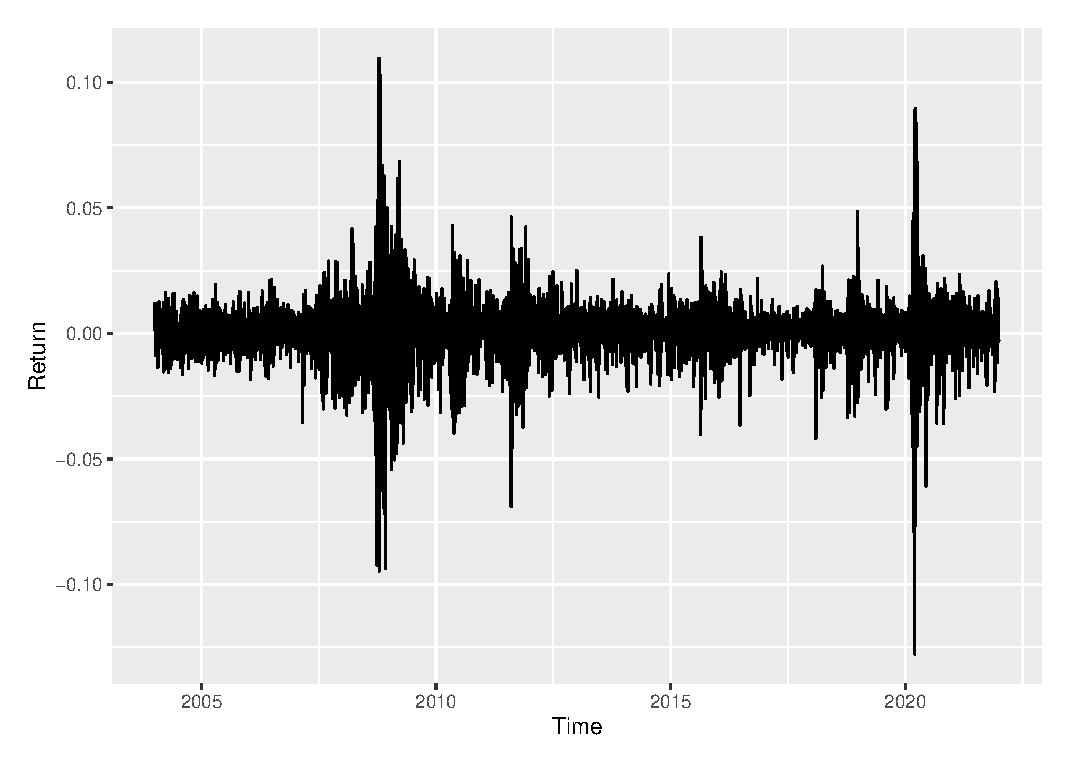
\includegraphics[width=0.9\textwidth]{Plots/Returns.eps}
\caption{Dynamics of the S\&P 500 market index log returns.}
\label{fig:plot_0}
\end{figure}

To ensure the robustness of the results, we estimated models both for the entire sample and for specific periods. It is important to consider that long financial time series may be characterized by structural breaks. Therefore, we decided to estimate the model on a set of samples that include observations of 3 years. The main goal of the analysis is to examine the S\&P 500 index for the asymmetric responses of risk premium to conditional volatility and compare the results of the GARCH-M-GJR-LEV model with alternatives by the Akaike information criterion. The estimation results for the whole sample and specific periods are presented in Tables \ref{tab:tab_4}-\ref{tab:tab_11}. The covariance matrix was estimated via the gradient outer product (GOP).

\subsection{Whole sample analysis}

In this subsection, we provide estimation results for all of the observations in the sample. In order to interpret the results meaningfully, it is necessary to evaluate all three models: GARCH-M, GARCH-M-GJR, and GARCH-M-GJR-LEV. Let's note that the GARCH-M model accounts for the risk premium effect, and GARCH-M-GJR captures the risk premium effect along with the leverage effect in the volatility equation. Finally, the proposed GARCH-M-GJR-LEV model allows accounting for the asymmetry effect both in volatility and risk premium responses to shocks in returns.  

\begin{table}[h!]
\caption{S\&P 500 estimation results for the period 2004-2021.}
\begin{center}
\label{tab:tab_4}
\begin{tabular*}{\textwidth}{cccc}
\hline
\hline
\multicolumn{1}{c}{\textbf{Parameters}} & \textbf{GARCH-M} & \textbf{GARCH-M-GJR} & \textbf{GARCH-M-GJR-LEV} \\
\hline
\hline

$\mu$                                      & 0.0499***        & 0.0225               & 0.0347**                 \\
                                        & (0.0141)         & (0.0138)             & (0.0140)                 \\
$\omega$                                   & 0.0286***        & 0.0287***            & 0.0291***                \\
                                        & (0.0024)         & (0.0020)             & (0.0012)                 \\
$\alpha$                                   & 0.1347***        & 0.0129***            & 0.0162***                \\
                                        & (0.0084)         & (0.0042)             & (0.0030)                 \\
$\beta$                                    & 0.8389***        & 0.8589***            & 0.8553***                \\
                                        & (0.0092)         & (0.0080)             & (0.0005)                 \\
$\lambda_{1}$                                  & 0.0265*          & 0.0135               & -0.0237***               \\
                                        & (0.0137)         & (0.0128)             & (0.0091)                 \\
$\gamma$                                   & -                & 0.1903***            & 0.1871***                   \\
                                        &                  & (0.0120)             & (0.0091)                 \\
$\lambda_{2}$                               & -                & -                    & 0.0760***                \\
                                        &                  &                      & (0.0003)                 \\
\hline
\textbf{AIC}                                     & \textbf{11791.596}            & \textbf{11643.245}                & \textbf{11629.996}                    \\
\hline
\hline
\end{tabular*}
\end{center}
\footnotesize
\renewcommand{\baselineskip}{11pt}
\textbf{Note:} *** —  $p<0.01$, ** —  $p < 0.05$, *– $p < 0.1$; st.errors in parentheses.
\end{table}


Based on the results presented in Table \ref{tab:tab_4}, all estimates in the GARCH-M-GJR-LEV model are statistically significant at any reasonable level. The parameters of most interest are $\lambda_{1}$ and $\lambda_{2}$. The estimate of $\lambda_{1}$ has a negative sign which is not intuitive since returns appear to react negatively to volatility increases. Although this coincides with the results found in previous research by \citep{Bollerslev2022}, such evidence may be caused by structural breaks. Therefore, we analyze this effect more carefully through the estimation of smaller samples in the next subsections. The estimate of $\lambda_{2}$ is positive and demonstrates that risk premium increases more sharply when volatility rises due to the negative shocks in returns. 

The asymmetric relationship between the risk premium and previous shocks in returns is visualized in Figure \ref{fig:plot_1}. Since the estimate of $\lambda_1$ is negative and the estimate of $\lambda_{2}$ is positive, therefore risk premium only rises when the observed shocks in returns are negative. This result clearly illustrates the above-mentioned contradictory findings and demonstrates that during ''good'' volatility periods, investors tend to demand a discount instead of a premium.

\begin{figure}[h!] %Figure 2
\centering
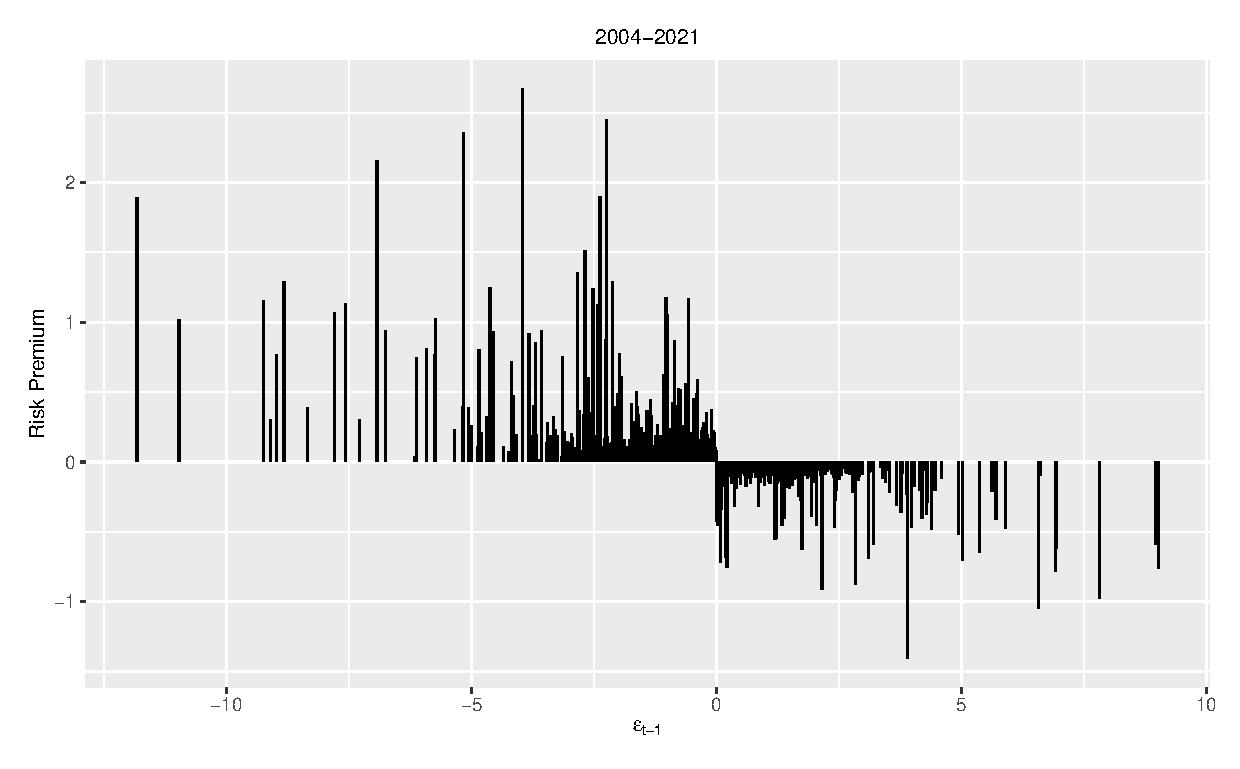
\includegraphics[width=0.85\textwidth]{Plots/Plot_whole.eps}
\caption{Risk premium responses to shocks in returns.}
\label{fig:plot_1}
\end{figure}

Comparing the results with the other two models, we see that estimate of $\lambda$ in the GARCH-M model is positive and statistically significant. Although, the absolute value of the effect is much smaller than in the GARCH-M-GJR model. Consequently, by estimating GARCH-M instead of the GARCH-M-GJR-LEV process, a researcher may underestimate the risk premium. Moreover, applying the GARCH-M-GJR model, we identify a significant estimate of the leverage effect in the volatility equation ($\gamma$), while the risk premium effect becomes insignificant and small. Therefore, by accounting for the leverage effect in the variance equation, one can misidentify the absence of the risk premium in returns since the leverage coefficient in the volatility equation takes on all the influence. Consequently, to properly identify the risk premium and leverage effects, the proposed GARCH-M-GJR-LEV model should be used because of the presence of an asymmetric risk premium effect in the observed data. Finally, the Akaike (AIC) criterion identifies the method as the best of all three options.

\subsection{Analysis of 3-year samples: 2019-2021, 2018-2020, 2017-2019}

This subsection provides results for the last three sequential 3-year samples. The estimation results are presented in Tables \ref{tab:tab_5}-\ref{tab:tab_7} correspondingly for each period. We combine these three periods into one subsection since they demonstrate similar results.

\begin{table}[h!]
\begin{center}
\caption{S\&P 500 estimation results for the period 2019-2021.}
\label{tab:tab_5}
\begin{tabular*}{\textwidth}{cccc}
\hline
\hline
\textbf{Parameters} & \textbf{GARCH-M}  & \textbf{GARCH-M-GJR} & \textbf{GARCH-M-GJR-LEV} \\
\hline
\hline
$\mu$                  & 0.0994***         & 0.0762**             & 0.0801**                 \\
                    & (0.032)           & (0.0319)             & (0.0327)                 \\
$\omega$               & 0.0656***         & 0.0718***            & 0.0711***                \\
                    & (0.0108)          & (0.0115)             & (0.0115)                 \\
$\alpha$               & 0.3034***         & 0.1623***            & 0.1616***                \\
                    & (0.0321)          & (0.0231)             & (0.023)                  \\
$\beta$                & 0.6777***         & 0.6569***            & 0.6574***                \\
                    & (0.0296)          & (0.0297)             & (0.0298)                 \\
$\lambda_{1}$              & 0.0325            & 0.0149               & -0.0114                  \\
                    & (0.0219)          & (0.019)              & (0.0271)                 \\
$\gamma$               & -                 & 0.3176***            & 0.3205***                \\
                    &                   & (0.0682)             & (0.0682)                 \\
$\lambda_{2}$           & -                 & -                    & 0.0644                   \\
                    &                   &                      & (0.0405)                 \\
\hline
\textbf{AIC}        & \textbf{2058.326} & \textbf{2046.602}    & \textbf{2046.535}        \\
\hline
\hline
\end{tabular*}
\end{center}
\footnotesize
\renewcommand{\baselineskip}{11pt}
\textbf{Note:} *** —  $p<0.01$, ** —  $p < 0.05$, *– $p < 0.1$; st.errors in parentheses.
\end{table}

\begin{table}[h!]
\begin{center}
\caption{S\&P 500 estimation results for the period 2018-2020.}
\label{tab:tab_6}
\begin{tabular*}{\textwidth}{cccc}
\hline
\hline
\textbf{Parameters} & \textbf{GARCH-M}  & \textbf{GARCH-M-GJR} & \textbf{GARCH-M-GJR-LEV} \\
\hline
\hline
$\mu$                  & 0.1017***         & 0.0780**             & 0.0829**                 \\
                    & (0.0314)          & (0.0328)             & (0.0328)                 \\
$\omega$               & 0.0550***         & 0.0533***            & 0.0522***                \\
                    & (0.0092)          & (0.0094)             & (0.0093)                 \\
$\alpha$               & 0.2467***         & 0.1390***            & 0.1399***                \\
                    & (0.0289)          & (0.0208)             & (0.0210)                 \\
$\beta$                & 0.7227***         & 0.7228***            & 0.7242***                \\
                    & (0.0274)          & (0.0261)             & (0.0260)                 \\
$\lambda_{1}$              & 0.0185            & 0.0060               & -0.0156                  \\
                    & (0.0242)          & (0.0224)             & (0.0097)                 \\
$\gamma$               & -                 & 0.2116***            & 0.2077***                \\
                    &                   & (0.0437)             & (0.0426)                 \\
$\lambda_{2}$           & -                 & -                    & 0.0489                   \\
                    &                   &                      & (0.0317)                 \\
\hline
\textbf{AIC}        & \textbf{2145.537} & \textbf{2132.454}    & \textbf{2133.173}        \\
\hline
\hline
\end{tabular*}
\end{center}
\footnotesize
\renewcommand{\baselineskip}{11pt}
\textbf{Note:} *** —  $p<0.01$, ** —  $p < 0.05$, *– $p < 0.1$; st.errors in parentheses.
\end{table}
All three periods are characterized by statistically insignificant and small estimates of $\lambda_{1}$ and $\lambda_{2}$ coefficients in the GARCH-M-GJR-LEV model. Consequently, we have found no statistical evidence of risk premium effects in the S\&P 500 returns on the analyzed periods. We should note that this finding coincides with the results of the GARCH-M and GARCH-M-GJR models because they do not capture a significant risk-premium effect either. The result is also reflected in the small difference in AIC criteria between GARCH-M-GJR and GARCH-M-GJR-LEV models. Nevertheless, it is crucial to account for the leverage effect in the variance equation since both GARCH-M-GJR and GARCH-M-GJR-LEV models provide significant and positive estimates of $\gamma$, which evidences that volatility appears to react more sharply on negative shocks in returns than on positive ones. This conclusion is supported by the great difference in the AIC criteria between the GARCH-M model and two other methods. Overall, the analyzed three periods are characterized by the absence of risk premium but include the leverage effect in the volatility equation, and, therefore, GARCH-M-GJR and the proposed GARCH-M-GJR-LEV model provide similar results.



\begin{table}[h!]
\begin{center}
\caption{S\&P 500 estimation results for the period 2017-2019.}
\label{tab:tab_7}
\begin{tabular*}{\textwidth}{cccc}
\hline
\hline
\textbf{Parameters} & \textbf{GARCH-M}  & \textbf{GARCH-M-GJR} & \textbf{GARCH-M-GJR-LEV} \\
\hline
\hline
$\mu$                  & 0.0911***         & 0.0616**             & 0.0566*                  \\
                    & (0.0300)          & (0.0291)             & (0.0301)                 \\
$\omega$               & 0.0306***         & 0.0287***            & 0.0298***                \\
                    & (0.0051)          & (0.0045)             & (0.0049)                 \\
$\alpha$               & 0.2022***         & 0.0106               & 0.0134                   \\
                    & (0.0258)          & (0.0204)             & (0.0218)                 \\
$\beta$                & 0.7561***         & 0.7910***            & 0.7808***                \\
                    & (0.0303)          & (0.0277)             & (0.0291)                 \\
$\lambda_{1}$              & 0.0390            & 0.0064               & 0.0243                   \\
                    & (0.0579)          & (0.0594)             & (0.0753)                 \\
$\gamma$               & -                 & 0.2856***            & 0.2928***                \\
                    &                   & (0.0357)             & (0.0387)                 \\
$\lambda_{2}$           & -                 & -                    & -0.0266                  \\
                        &                   &             & (0.0789)                     \\
\hline
\textbf{AIC}        & \textbf{1538.754} & \textbf{1500.615}    & \textbf{1502.444}        \\
\hline
\hline
\end{tabular*}
\end{center}
\footnotesize
\renewcommand{\baselineskip}{11pt}
\textbf{Note:} *** —  $p<0.01$, ** —  $p < 0.05$, *– $p < 0.1$; st.errors in parentheses.
\end{table}

\subsection{Analysis of 3-year samples: 2016-2018, 2015-2017, 2014-2016, 2013-2015}

In this subsection, we discuss results obtained from the analysis of four sequential 3-year samples, covering the period from 2013 to 2018. The estimation results of all periods are presented in Tables \ref{tab:tab_8}-\ref{tab:tab_11}. As with the previous case, this section merges periods with similar patterns.

Based on the presented results, all estimated periods demonstrate statistically significant estimates of $\lambda_{2}$ parameter in the GARCH-M-GJR-LEV model. The result provides evidence that returns include the asymmetric relationship between the risk-premium and shocks in returns. The estimate is positive among all the estimated periods. Consequently, this clearly represents that risk premium increases more sharply when volatility rises due to negative shocks in returns rather than positive ones. This evidence supports the ''bad'' and ''good'' volatility differentiation hypothesis of \citep{Bollerslev2022}. That is, investors tend to demand a higher risk premium during the ''bear'' market, i.e., driven by ''bad'' volatility than in the case of ''good'' volatility periods.

\begin{table}[h!]
\begin{center}
\caption{S\&P 500 estimation results for the period 2016-2018.}
\label{tab:tab_8}
\begin{tabular*}{\textwidth}{cccc}
\hline
\hline
\textbf{Parameters} & \textbf{GARCH-M}  & \textbf{GARCH-M-GJR} & \textbf{GARCH-M-GJR-LEV} \\
\hline
\hline
$\mu$                  & 0.0598**          & 0.0301               & 0.0470                   \\
                    & (0.0297)          & (0.0304)             & (0.0301)                 \\
$\omega$               & 0.0394***         & 0.0370***            & 0.0344***                \\
                    & (0.0057)          & (0.0054)             & (0.0051)                 \\
$\alpha$               & 0.2146***         & 0.0507***            & 0.0581***                \\
                    & (0.0213)          & (0.0143)             & (0.0171)                 \\
$\beta$                & 0.7382***         & 0.7634***            & 0.7701***                \\
                    & (0.0297)          & (0.0284)             & (0.0288)                 \\
$\lambda_{1}$              & 0.0424            & 0.0319               & -0.0749                  \\
                    & (0.0573)          & (0.0544)             & (0.0525)                 \\
$\gamma$               & -                 & 0.2556***            & 0.2527***                \\
                    &                   & (0.0298)             & (0.0398)                 \\
$\lambda_{2}$           & -                 & -                    & 0.1914***                \\
                    &                   &                     & (0.0483)                 \\
\hline
\textbf{AIC}        & \textbf{1575.468} & \textbf{1557.305}    & \textbf{1553.541}        \\
\hline
\hline
\end{tabular*}
\end{center}
\footnotesize
\renewcommand{\baselineskip}{11pt}
\textbf{Note:} *** —  $p<0.01$, ** —  $p < 0.05$, *– $p < 0.1$; st.errors in parentheses.
\end{table}

According to Table \ref{tab:tab_8}, the estimate of $\lambda_{1}$ in the GARCH-M model is statistically insignificant, while the GARCH-M-GJR-LEV model provides a significant estimate of $\lambda_{2}$. It is an important result since it demonstrates that the GARCH-M model was not able to capture a risk premium at all, while GARCH-M-GJR-LEV has identified it. Taking into account that estimate of $\lambda_{1}$ in the proposed method is also statistically insignificant, we can conclude that the risk premium in the S\&P 500 returns on this period reacts only to 'bad' volatility, while 'bull' market volatility fluctuations do not increase the risk premium. In other words, investors appear to demand risk premiums only during the drops in financial markets. In contrast, high market turbulence during periods of sharp growth does not stimulate an investor to require a higher risk premium. This pattern demonstrates the irrationality of investors: one appears to perceive negative news more dramatically in comparison with positive ones. Such evidence is consistent with the prospect theory of \citep{Kahneman1979} and \citep{Zhang2006}, \citep{Black1976}, \citep{Nelson1991}.


Besides that, it is important to note that the data is also characterized by asymmetric volatility responses to shocks in returns since GARCH-M-GJR and GARCH-M-GJR-LEV models demonstrate significant and positive estimates of $\gamma$. We may also see it from lower values of AIC criteria in asymmetric models compared to the GARCH-M model. 

Finally, the proposed GARCH-M-GJR-LEV model appears to be the best based on the Akaike information criteria. In other words, the model allowed to capture both leverage effects and, consequently, ensured a higher accuracy of estimation.\footnote{Leverage effects in return and volatility equations.} Furthermore, since the GARCH-M model did not capture a significant risk premium effect, one may misidentify the presence of risk premium in the returns without applying the GARCH-M-GJR-LEV model.

Further, Tables \ref{tab:tab_9}-\ref{tab:tab_11} represent similar results. The only difference in these periods is that the estimate of $\lambda_{1}$ coefficient in the GARCH-M model is statistically significant in all three tables. This means that the GARCH-M model was able to capture a risk-premium effect in contrast to the 2016-2018 period. Besides that, it is crucial to analyze the estimation results provided by the GARCH-M-GJR model. It is clearly seen that among all three tables, after accounting for the asymmetry in the variance equation (through the application of the GARCH-M-GJR model), the estimate of $\lambda_{1}$ becomes statistically insignificant. That is, a researcher may not be able to capture the risk premium by estimating the GJR specification. As a consequence, this may lead to a substantial misinterpretation of the results.

Further, as with the 2016-2017 results, the estimate of $\lambda_{1}$ in the GARCH-M-GJR-LEV model is statistically insignificant (Tables \ref{tab:tab_9}-\ref{tab:tab_11}). This evidences again that investors demand a risk premium only during ''bad'' volatility periods when variance rises due to the sharp falls in returns.

\begin{table}[h!]
\begin{center}
\caption{S\&P 500 estimation results for the period 2015-2017.}
\label{tab:tab_9}
\begin{tabular*}{\textwidth}{cccc}
\hline
\hline
\textbf{Parameters} & \textbf{GARCH-M}  & \textbf{GARCH-M-GJR} & \textbf{GARCH-M-GJR-LEV} \\
\hline
\hline
$\mu$                  & 0.0004            & 0.0011               & 0.0065                   \\
                    & (0.0313)          & (0.0312)             & (0.0164)                 \\
$\omega$               & 0.0464***         & 0.0492***            & 0.0497***                \\
                    & (0.0068)          & (0.0086)             & (0.0085)                 \\
$\alpha$               & 0.2401***         & 0.0543***            & 0.0589***                \\
                    & (0.0218)          & (0.0134)             & (0.0125)                 \\
$\beta$                & 0.6996***         & 0.7107***            & 0.7003***                \\
                    & (0.0329)          & (0.0403)             & (0.0398)                 \\
$\lambda_{1}$              & 0.1664**          & 0.0892               & 0.0134                   \\
                    & (0.0650)          & (0.0594)             & (0.0324)                 \\
$\gamma$               & -                 & 0.3065***            & 0.3098***                \\
                    &                   & (0.0352)             & (0.0351)                 \\
$\lambda_{2}$           & -                 & -                    & 0.1792***                \\
                    &                   &                      & (0.0486)                 \\
\hline
\textbf{AIC}        & \textbf{1553.335} & \textbf{1531.684}    & \textbf{1523.906}        \\
\hline
\hline
\end{tabular*}
\end{center}
\footnotesize
\renewcommand{\baselineskip}{11pt}
\textbf{Note:} *** —  $p<0.01$, ** —  $p < 0.05$, *– $p < 0.1$; st.errors in parentheses.
\end{table}


\begin{table}[h!]
\begin{center}
\caption{S\&P 500 estimation results for the period 2014-2016.}
\label{tab:tab_10}
\begin{tabular*}{\textwidth}{cccc}
\hline
\hline
\textbf{Parameters} & \textbf{GARCH-M}  & \textbf{GARCH-M-GJR} & \textbf{GARCH-M-GJR-LEV} \\
\hline
\hline
$\mu$                  & 0.0004            & 0.0004               & 0.0004                   \\
                    & (0.0422)          & (0.0397)             & (0.0419)                 \\
$\omega$               & 0.0691***         & 0.0703***            & 0.0679***                \\
                    & (0.0123)          & (0.0137)             & (0.0139)                 \\
$\alpha$               & 0.2499***         & 0.0233               & 0.0058                   \\
                    & (0.0262)          & (0.0152)             & (0.0174)                 \\
$\beta$                & 0.6874***         & 0.6996***            & 0.7172***                \\
                    & (0.0399)          & (0.0454)             & (0.0461)                 \\
$\lambda_{1}$              & 0.1435**          & 0.0578               & -0.0049                  \\
                    & (0.0656)          & (0.0577)             & (0.0635)                 \\
$\gamma$               & -                 & 0.3630***            & 0.3711***                \\
                    &                   & (0.0429)             & (0.0402)                 \\
$\lambda_{2}$           & -                 & -                    & 0.1826**                 \\
                    &                   &                      & (0.0747)        \\
\hline
\textbf{AIC}        & \textbf{1753.369} & \textbf{1720.883}    & \textbf{1715.978}        \\
\hline
\hline
\end{tabular*}
\end{center}
\footnotesize
\renewcommand{\baselineskip}{11pt}
\textbf{Note:} *** —  $p<0.01$, ** —  $p < 0.05$, *– $p < 0.1$; st.errors in parentheses.
\end{table}

The estimate of the leverage effect ($\gamma$) in the variance equation is significant among all periods. This result is consistent not only between the GARCH-M-GJR and GARCH-M-GJR-LEV models but also across periods. Consequently, it reveals that the S\&P 500 index returns exhibit the asymmetry effect, which should be properly captured to provide a better quality of estimation. 

\begin{table}[h!]
\begin{center}
\caption{S\&P 500 estimation results for the period 2013-2015.}
\label{tab:tab_11}
\begin{tabular*}{\textwidth}{cccc}
\hline
\hline
\textbf{Parameters} & \textbf{GARCH-M}  & \textbf{GARCH-M-GJR} & \textbf{GARCH-M-GJR-LEV} \\
\hline
\hline
$\mu$                  & 0.0042            & 0.0041               & 0.0174                   \\
                    & (0.0514)          & (0.0387)             & (0.0282)                 \\
$\omega$               & 0.0750***         & 0.0683***            & 0.0631***                \\
                    & (0.0194)          & (0.0159)             & (0.0144)                 \\
$\alpha$               & 0.1973***         & 0.0002               & 0.0003                   \\
                    & (0.0374)          & (0.0379)             & (0.0069)                 \\
$\beta$                & 0.6854***         & 0.6954***            & 0.7039***                \\
                    & (0.0524)          & (0.0493)             & (0.0461)                 \\
$\lambda_{1}$              & 0.1671*           & 0.0794               & 0.0123                   \\
                    & (0.0877)          & (0.0625)             & (0.0715)                 \\
$\gamma$               & -                 & 0.3996***            & 0.3915***                \\
                    &                   & (0.0588)             & (0.0411)                 \\
$\lambda_{2}$           & -                 & -                    & 0.1477***                \\
                    &                   &                      & (0.0476)                 \\
\hline
\textbf{AIC}        & \textbf{1700.135} & \textbf{1651.677}    & \textbf{1650.606}        \\
\hline
\hline
\end{tabular*}
\end{center}
\footnotesize
\renewcommand{\baselineskip}{11pt}
\textbf{Note:} *** —  $p<0.01$, ** —  $p < 0.05$, *– $p < 0.1$; st.errors in parentheses.
\end{table}

\begin{figure}[h!] %Figure 3
\centering
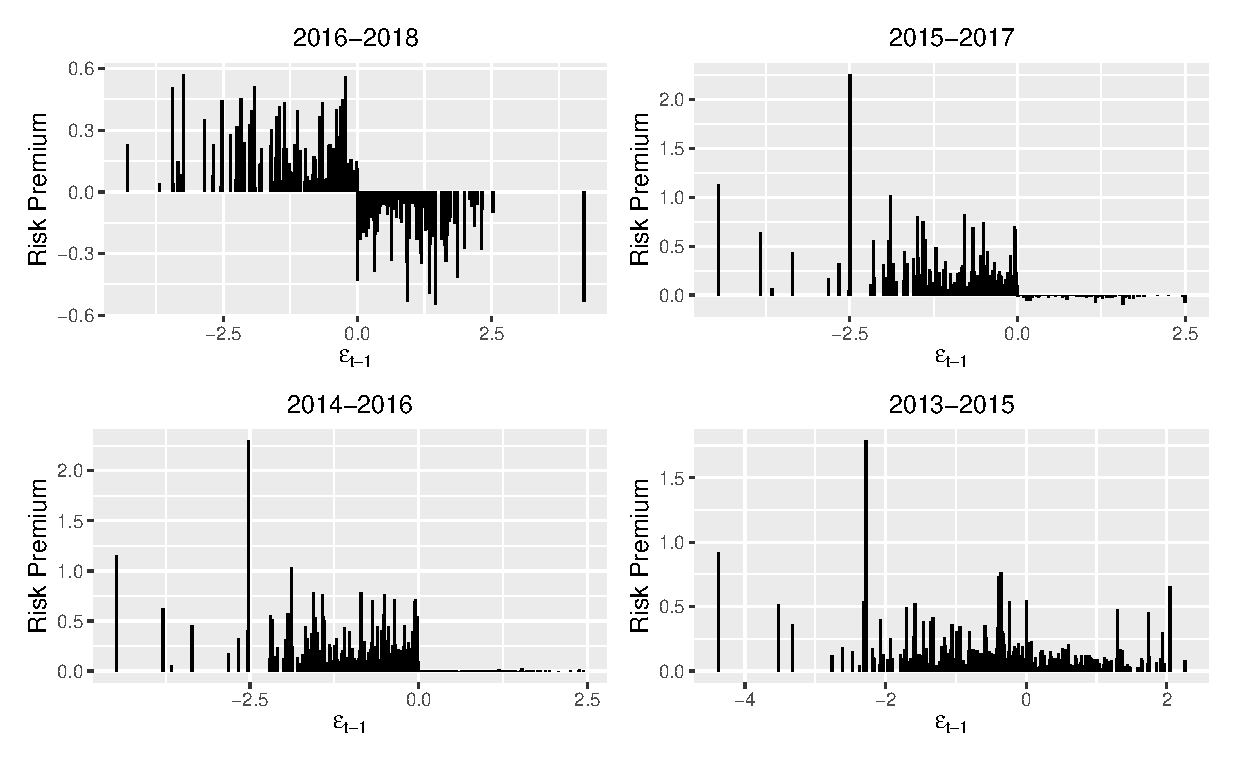
\includegraphics[width=0.85\textwidth]{Plots/Plot_periods.eps}
\caption{Risk premium responses to shocks in returns.}
\label{fig:plot_2}
\end{figure}

In Figure \ref{fig:plot_2}, we present the dependence of the risk premium on previous values of shocks in returns for each period. All periods demonstrate an asymmetric relationship between the risk premium and volatility changes, based on the sign of shocks that cause volatility rises. The graph for the period 2016-2018 represents a similar pattern to the whole sample dependence (Figure \ref{fig:plot_1}), while three other periods exhibit a different structure. The difference is explained only by the sign of the $\lambda_1$ estimate. Because it was negative and high for the period 2016-2018 (relative to other periods), thus the plot illustrates that investors demand a risk premium only during ''bad'' volatility periods, while ''good'' volatility may even produce a discount. The period 2015-2017 also illustrates that the risk premium is negative (risk discount) when shocks in returns are positive ones, albeit the absolute discount value is significantly lower compared to 2016-2018. It is due to the lower estimate value of $\lambda_1$. The remaining two periods demonstrate that risk premium rises during both ''good'' and ''bad'' volatility periods, while negative shocks in returns influence the premium more sharply, i.e., investors demand a higher risk premium during the ''bear'' market.

To sum up, there has been found statistical evidence that the observed data exhibit both the asymmetry effect in the variance equation and asymmetric responses of the risk premium to volatility changes. The proposed GARCH-M-GJR-LEV method allows capturing both of these effects simultaneously. Because of this integral feature, the model was able to provide a better estimation quality, which is justified by the lower values of the AIC information criterion.



\section{Results \& Conclusion}

In this study, we have proposed the GARCH-M-GJR-LEV model. Its integral feature is to account for asymmetric responses in the return and variance equations simultaneously. According to \citep{Bollerslev2022}, investors perceive ''good'' and ''bad'' volatility periods differently, demanding different risk premiums. While well-known asymmetric GARCH models (e.g., EGARCH and GJR-GARCH) capture asymmetric responses of variance to shocks in returns, they either do not account for a risk premium at all or assume that it reacts equally to negative and positive return fluctuations. In contrast, the proposed method distinguishes between volatility caused by the ''bear'' and ''bull'' markets while modeling the risk premium.

We have derived the specification of unconditional variance for the proposed method and studied the properties via the simulated data analysis. According to the results, the GARCH-M-GJR-LEV model demonstrates a significant advantage compared with other methods, in case the data generating process is characterized by an asymmetric relationship between the risk premium and volatility changes. Therefore without applying the model, one may obtain inaccurate estimates of GARCH model parameters, conditional volatilities, and returns.

Further, the introduced model was applied to study the volatility of the S\&P 500 market index. As a result, we have found statistical evidence in favor of the presence of the leverage effect in the mean equation over various time periods. Consequently, investors demand a higher risk premium in case volatility is determined by negative shocks in returns rather than positive ones. Moreover, the results indicate that only negative shocks tend to form a risk premium during some time intervals. In other words, investors demanded a risk premium only during ''bad'' volatility periods. This evidence coincides with other empirical results \citep{Bollerslev2006}, \citep{Rossi2015}, and the prospect theory of \citep{Kahneman1979}. Furthermore, we have found that a researcher may not be able to properly estimate a risk premium without applying the GARCH-M-GJR-LEV model in case the data demonstrate a leverage effect in the return equation. This problem may lead to a significant misinterpretation of results. Finally, the Akaike information criterion indicates that the proposed model appears to be the best among alternatives during most of the periods.

\bibliographystyle{elsarticle-harv} 
\bibliography{library}

\appendix
\section{Derivation of the unconditional variance}

Here we derive an expression for the unconditional variance of returns, i.e., $Var\left(y_{t}\right)$. 

\newproof{pot}{Proof of Theorem \ref{thm:thm_1}}
\newproof{pf}{Proof}

\begin{pot}

First, let's derive some preliminary results.
Remind that from \citet{Glosten1993}:
\begin{equation}\label{eq:r0}
Var\left(\varepsilon_{t}\right) = \mathbb{E}\left[\varepsilon^2_{t}\right] = \mathbb{E}\left[\sigma^{2}_{t}\right]=\frac{\omega}{1 - \alpha - \beta - \frac{1}{2}\gamma}.
\end{equation}

Notice that $I_{t}=I_{t}^{s}$ for any $s\in N$ and $\sigma_{t}$ is independent of $\xi_{t}$, so:

\begin{equation}\label{eq:r1}
\mathbb{E}\left[I_{t}^{2}\sigma^{2}_{t}\right]=\mathbb{E}\left[I_{t}\sigma^{2}_{t}\right]=\mathbb{E}\underbrace{\left[\sigma^{2}_{t}|\xi_{t}<0\right]}_{\text{independent}} \times P\left(\xi_{t}<0\right)=\frac{1}{2}\mathbb{E}\left[\sigma^{2}_{t}\right],
\end{equation}

\begin{equation}\label{eq:r2}
\mathbb{E}\left[I_{t}^{2}\sigma^{4}_{t}\right]=\mathbb{E}\left[I_{t}\sigma^{4}_{t}\right]=\mathbb{E}\underbrace{\left[\sigma^{4}_{t}|\xi_{t}<0\right]}_{\text{independent}} \times P\left(\xi_{t}<0\right)=\frac{1}{2}\mathbb{E}\left[\sigma^{4}_{t}\right].
\end{equation}

Using the first and the fourth moments of a standard normal distribution, we get:

\begin{equation}\label{eq:r3}
\mathbb{E}\left[\varepsilon_{t}^{2}\right]=\mathbb{E}\left[\sigma_{t}^2\xi_{t}^2\right]=\mathbb{E}\left[\sigma_{t}^2\right] \times \mathbb{E}\left[\xi_{t}^2\right]=\mathbb{E}[\sigma^2_{t}],
\end{equation}

\begin{equation}\label{eq:r4}
\mathbb{E}\left[\varepsilon_{t}^{4}\right]=\mathbb{E}\left[\sigma_{t}^4\xi_{t}^4\right]=\mathbb{E}\left[\sigma_{t}^4\right] \times \mathbb{E}\left[\xi_{t}^4\right]=3\mathbb{E}\left[\sigma^4_{t}\right].
\end{equation}

Simply expanding the expression of shocks, one gets:

\begin{equation}\label{eq:r5}
\mathbb{E}\left[\varepsilon_{t}^{2}\sigma_{t}^{2}\right]=\mathbb{E}\left[\sigma^{2}_{t}\xi^{2}_{t}\sigma_{t}^{2}\right]=\mathbb{E}\left[\sigma_{t}^4\right].
\end{equation}

The distribution of $\xi^2_{t}$ does not depend on the event $\xi_{t}<0$ if $\xi_{t}$ is symmetric around zero, which is the case of a standard normal distribution, so:

\begin{equation}\label{eq:r6}
\mathbb{E}\left[I_{t}\varepsilon_{t}^{2}\right]=\mathbb{E}\underbrace{\left[\sigma_{t}^2\xi_{t}^2|\xi_{t} < 0\right]}_{\text{independent}} \times P\left(\xi < 0\right)=\frac{1}{2}\mathbb{E}\left[\sigma^2_{t}\right] \times \mathbb{E}\left[\xi^2_{t}\right]=\frac{1}{2}\mathbb{E}\left[\sigma^2_{t}\right],
\end{equation}

\begin{equation}\label{eq:r7}
\mathbb{E}\left[I_{t}\varepsilon_{t}^{4}\right]=\mathbb{E}\underbrace{\left[\sigma_{t}^4\xi_{t}^4|\xi_{t} < 0\right]}_{\text{independent}}\times P\left(\xi < 0\right)=\frac{1}{2}\mathbb{E}\left[\sigma^4_{t}\right] \times \mathbb{E}\left[\xi^4_{t}\right]=\frac{3}{2}\mathbb{E}\left[\sigma^4_{t}\right],
\end{equation}
\begin{align}\label{eq:r8}
\begin{split}
\mathbb{E}\left[I_{t} \sigma_{t}^2 \varepsilon_{t}^2\right] = \mathbb{E}\left[I_{t} \sigma_{t} ^ 4 \xi_{t} ^ 2\right] & = \mathbb{E}\left[\sigma_{t} ^ 4 \xi_{t} ^ 2|\xi_{t} < 0\right] \times P\left(\xi_{t} < 0\right)= \\ 
& = \frac{1}{2}\mathbb{E}\left[\sigma_{t} ^ 4\right] \times \mathbb{E}\left[\xi_{t} ^ 2\right]=\frac{1}{2}\mathbb{E}\left[\sigma_{t} ^ 4\right].
\end{split}
\end{align}

Using the aforementioned formulas, it is straightforward to show that:

\begin{align} \label{eq:r9}
\begin{split}
\mathbb{E}\left[\sigma^{4}_{t}\right] & =\mathbb{E}\left[\left(\omega + \alpha \varepsilon^{2}_{t-1}+\beta \sigma^{2}_{t-1}+\gamma I_{t-1} \varepsilon^{2}_{t-1}\right)^2\right]= \\
& = \omega^2 + \alpha ^ 2 \mathbb{E}\left[\varepsilon_{t-1} ^ 4\right] + \beta ^ 2 \mathbb{E}\left[\sigma^{4}_{t - 1}\right] + \\
& \;\;\;\; + \gamma ^ 2 \mathbb{E}\left[I^{2}_{t-1}\varepsilon^{4}_{t-1}+2\omega\alpha \mathbb{E}\left[\varepsilon^{2}_{t-1}\right] + 2\omega\beta \mathbb{E}\left[\sigma^{2}_{t-1}\right]\right] + 2\omega\gamma \mathbb{E}\left[I_{t-1} \varepsilon^{2}_{t-1}\right] + \\
& \;\;\;\; + 2\alpha\beta \mathbb{E}\left[\varepsilon^{2}_{t-1}\sigma^{2}_{t-1}\right]+ 2\alpha\gamma \mathbb{E}\left[I_{t-1}\varepsilon^{4}_{t-1}\right] + 2\beta\gamma \mathbb{E}\left[I_{t-1} \sigma^{2}_{t-1} \varepsilon^{2}_{t-1}\right] = \\
& =\omega^2+\left(3\alpha ^ 2 + \beta^2 + \frac{3}{2}\gamma ^ 2 + 2\alpha\beta + 3\alpha\gamma +\beta\gamma\right) \times \mathbb{E}\left[\sigma_{t}^4\right] + \\  & \;\;\;\; + \omega \mathbb{E}\left[\sigma^2_{t}\right] \times \left(2\alpha + 2\beta + \gamma\right).
\end{split}
\end{align}

Solving for $\mathbb{E}\left[\sigma_{t}^4\right]$, we get:
\begin{align}\label{eq:r10}
\mathbb{E}\left[\sigma_{t}^4\right] = \frac{\omega^2 + \omega \mathbb{E}\left[\sigma^2_{t}\right] \times (2\alpha + 2\beta + \gamma)}{1 - 3\alpha ^ 2 - \beta^2 - \frac{3}{2}\gamma ^ 2 - 2\alpha\beta - 3\alpha\gamma - \beta\gamma}.
\end{align}

Now we are ready to derive the expression for the unconditional variance of $y_{t}$:
\begin{align} \label{eq:r11}
\begin{split}
\sigma^2=Var(y_{t}) & =Var\left(\mu+\lambda_{1}\sigma^{2}_{t-1}+\lambda_{2} I_{t-1}\sigma^{2}_{t-1}+\varepsilon_{t}\right)= \\
& =Var\left(\lambda_{1}\sigma^{2}_{t-1}+\lambda_{2} I_{t-1}\sigma^{2}_{t-1}\right) + Var\left(\varepsilon_{t}\right) + \\
& \;\;\;\; + 2\underbrace{Cov\left(\lambda_{1}\sigma^{2}_{t-1}+\lambda_{2} I_{t-1}\sigma^{2}_{t-1},\varepsilon_{t}\right)}_{\text{zero because of independence}}= \\
& =\lambda_{1}^2Var\left(\sigma^{2}_{t-1}\right)+\lambda_{2}^2Var\left(I_{t-1}\sigma^{2}_{t-1}\right)+ \\
& \;\;\;\; + 2\lambda_{1}\lambda_{2}Cov\left(\sigma^{2}_{t-1}, I_{t-1}\sigma^{2}_{t-1}\right)+\mathbb{E}\left[\sigma^2_{t}\right] = \\
& =\lambda_{1}^2 \times \left(\mathbb{E}\left[\sigma^4_{t-1}\right]-\mathbb{E}\left[\sigma^2_{t-1}\right]^2\right) + \\
& \;\;\;\; + \frac{1}{2} \lambda_{2}^2 \times \left(\mathbb{E}\left[\sigma^4_{t-1}\right] - \frac{1}{2} \mathbb{E}\left[\sigma^2_{t-1}\right]^2\right) + \\
& \;\;\;\; + \lambda_{1} \lambda_{2} \times \left(\mathbb{E}\left[\sigma^4_{t-1}\right] - \mathbb{E}\left[\sigma^2_{t-1}\right]^2\right) + \mathbb{E}\left[\sigma^2_{t}\right].
\end{split}
\end{align}

Note that since the process is stationary, then $\mathbb{E}\left[\sigma^4_{t-1}\right] = \mathbb{E}\left[\sigma^4_{t}\right]$ and $\mathbb{E}\left[\sigma^2_{t-1}\right] = \mathbb{E}\left[\sigma^2_{t}\right]$. Applying this and simplifying the expression, the final specification of the unconditional variance in the GARCH-M-GJR-LEV process takes the following form:
\begin{align}\label{eq:r12}
\begin{split}
Var\left(y_{t}\right) & =\left(\lambda_{1}^2 + \lambda_{1} \lambda_{2}\right) \times \left(\mathbb{E}\left[\sigma^4_{t}\right] - \mathbb{E}\left[\sigma^2_{t}\right]^2\right) + \\ & \;\;\;\; + \frac{1}{2} \lambda^2_{2} \times \left(\mathbb{E}\left[\sigma^4_{t}\right] - \frac{1}{2} \mathbb{E}\left[\sigma^2_{t}\right]^2\right) + \mathbb{E}\left[\sigma^2_{t}\right],
\end{split}
\end{align}
where $\mathbb{E}\left[\sigma_{t}^2\right]$ and $\mathbb{E}\left[\sigma_{t}^4\right]$ can be calculated by the formulas (\ref{eq:r0}) and (\ref{eq:r10}) correspondingly.
\end{pot}
\hfill$\square$
 
Additionally, using the above-mentioned formulas, it is possible to show that the unconditional variance of $\sigma^2_{t}$ is specified as follows:
\begin{align}
\begin{split}
Var(\sigma^2_{t}) & = \Bigl(\alpha^2 \times \left(3\mathbb{E}\left[\sigma^4_{t}\right] - \mathbb{E}{\left[\sigma^2_{t}\right]}^2 \right) + 2 \alpha \beta \times \left(\mathbb{E}\left[\sigma^4_{t}\right] - \mathbb{E}{\left[\sigma^2_{t}\right]}^2 \right) + \\ 
& \;\;\;\; + \gamma^2 \times \left(\frac{3}{2} \mathbb{E}[\sigma^4_{t}] - 
\frac{1}{4} \mathbb{E}{\left[\sigma^2_{t}\right]}^2 \right) +  \alpha \gamma \times \left(3\mathbb{E}[\sigma^4_{t}] - \mathbb{E}{\left[\sigma^2_{t}\right]}^2 \right) + \\
& \;\;\;\; + \beta \gamma \times \left(\mathbb{E}[\sigma^4_{t}] - \mathbb{E}{\left[\sigma^2_{t}\right]}^2 \right)\Bigr) \times \Bigl(1 - \beta^2 \Bigr) ^ {-1}.
 \end{split}
\end{align}

 \newpage
 
\section{Alternative metrics for model comparison.}

In this Section, we provide the calculated values of MAE and MSE accuracy metrics for parameter estimates, conditional volatilities, and returns. Tables \ref{tab:ap_5}-\ref{tab:ap_8}, similarly to RMSE, demonstrate the advantage of the GARCH-M-GJR-LEV model over alternative methods.

\begin{table}[h!]
\centering
\caption{Simulation 1.}
\label{tab:ap_5}
\begin{tabular}{lccc}
\hline
\hline
\textbf{Metric/Model}    & \textbf{GARCH-M} & \textbf{GARCH-M-GJR} & \textbf{GARCH-M-GJR-LEV} \\
$MAE(\hat{\mu})$           & 5.047                             & 4.247                                  & 2.608                                       \\
$MAE(\hat{\omega})$        & 2.501                             & 2.281                                  & 2.092                                       \\
$MAE(\hat{\alpha})$        & 9.239                             & 3.014                                  & 2.908                                       \\
$MAE(\hat{\beta})$         & 4.481                             & 4.120                                  & 4.143                                       \\
$MAE(\hat{\lambda}_1)$       & 19.959                            & 5.473                                  & 5.340                                       \\
$MAE(\hat{\gamma})$        & -                                 & 21.676                                 & 5.341                                       \\
$MAE(\hat{\lambda}_2)$    & -                                 & -                                      & 5.879                                       \\

\hline

$MSE(\hat{\mu})$           & 0.500                             & 0.364                                  & 0.211                                       \\
$MSE(\hat{\omega})$        & 0.114                             & 0.096                                  & 0.067                                       \\
$MSE(\hat{\alpha})$        & 1.020                             & 0.159                                  & 0.170                                       \\
$MSE(\hat{\beta})$         & 0.374                             & 0.343                                  & 0.289                                       \\
$MSE(\hat{\lambda}_1)$       & 4.589                             & 0.581                                  & 0.438                                       \\
$MSE(\hat{\gamma})$        & -                                 & 5.246                                  & 0.421                                       \\
$MSE(\hat{\lambda}_2)$    & -                                 & -                                     & 0.790    \\

\hline
\hline                                  
\end{tabular}
\end{table}

\begin{table}[h!]
\centering
\caption{Simulation 2.}
\label{tab:ap_6}
\begin{tabular}{lccc}
\hline
\hline
\textbf{Metric/Model}    & \textbf{GARCH-M} & \textbf{GARCH-M-GJR} & \textbf{GARCH-M-GJR-LEV} \\

$MAE(\hat{\mu})$           & 3.537                             & 2.766                                  & 2.754                                       \\
$MAE(\hat{\omega})$        & 1.725                             & 1.357                                  & 1.377                                       \\
$MAE(\hat{\alpha})$        & 12.245                            & 2.528                                  & 2.580                                       \\
$MAE(\hat{\beta})$         & 4.772                             & 3.174                                  & 3.299                                       \\
$MAE(\hat{\lambda}_1)$       & 13.063                            & 26.252                                 & 25.080                                      \\
$MAE(\hat{\gamma})$        & -                             & 14.681                                 & 23.254                                      \\
$MAE(\hat{\lambda}_2)$    & -                             & -                                  & 5.472                                       \\
\hline
$MSE(\hat{\mu})$            & 0.176                             & 0.108                                  & 0.114                                       \\
$MSE(\hat{\omega})$        & 0.099                             & 0.029                                  & 0.029                                       \\
$MSE(\hat{\alpha})$        & 1.645                             & 0.096                                  & 0.100                                       \\
$MSE(\hat{\beta})$         & 0.505                             & 0.168                                  & 0.157                                       \\
$MSE(\hat{\lambda}_1)$       & 1.980                             & 7.163                                  & 6.552                                       \\
$MSE(\hat{\gamma})$        & -                             & 2.344                                  & 5.745                                       \\
$MSE(\hat{\lambda}_2)$    & -                             & -                                  & 0.490 \\
\hline
\hline                                       
\end{tabular}
\end{table}

\begin{table}[h!]
\centering
\caption{Sim 1).}
\label{tab:ap_7}
\begin{tabular}{cccc}
\hline
\hline
\textbf{Metric/Model} & \multicolumn{1}{l}{\textbf{GARCH-M}} & \multicolumn{1}{l}{\textbf{GARCH-M-GJR}} & \multicolumn{1}{l}{\textbf{GARCH-M-GJR-LEV}} \\
$MAE(\hat{\sigma})$   & 7.655         & 6.237              & 3.694                   \\
$MSE(\hat{\sigma})$   & 1.524         & 1.060              & 0.377                   \\
$MAE(\hat{y})$     & 71.677        & 71.453             & 69.117                  \\
$MSE(\hat{y})$     & 89.456        & 88.755             & 82.025                  \\
\hline 
\hline
\end{tabular}
\end{table}

\begin{table}[h!]
\centering
\caption{Sim 2).}
\label{tab:ap_8}
\begin{tabular}{cccc}
\hline
\hline
\textbf{Metric/Model} & \multicolumn{1}{l}{\textbf{GARCH-M}} & \multicolumn{1}{l}{\textbf{GARCH-M-GJR}} & \multicolumn{1}{l}{\textbf{GARCH-M-GJR-LEV}} \\
$MAE(\hat{\sigma})$   & 9.161         & 4.478              & 3.957                   \\
$MSE(\hat{\sigma})$   & 1.766         & 0.481            & 0.337                  \\
$MAE(\hat{y})$     & 74.851        & 74.763             & 74.032                  \\
$MSE(\hat{y})$     & 100.787        & 100.572             & 97.548                  \\
\hline 
\hline
\end{tabular}
\end{table}



\section{Robustness to normality assumption violation}

Here we provide the results for the QMLE estimators. Tables \ref{tab:ap_1}-\ref{tab:ap_2} present the results assuming the Student's distribution, while Tables \ref{tab:ap_3}-\ref{tab:ap_4} reflect the results assuming the Non-central Student's distribution.

\begin{table}[h!]
\centering
\caption{Accuracy metrics of coefficient estimates (Student's distribution).}
\label{tab:ap_1}
\begin{tabular}{lccc}
\hline
\hline
\textbf{Metric/Model}    & \textbf{GARCH-M} & \textbf{GARCH-M-GJR} & \textbf{GARCH-M-GJR-LEV} \\
$RMSE(\hat{\mu})$        & 8.961    & 7.596    & 5.076  \\
$RMSE(\hat{\omega})$     & 5.962    & 3.881    & 3.275  \\
$RMSE(\hat{\alpha})$     & 10.866   & 4.709    & 3.935  \\
$RMSE(\hat{\beta})$      & 8.679    & 6.944    & 6.245  \\
$RMSE(\hat{\lambda}_1)$  & 20.727   & 8.462    & 7.262  \\
$RMSE(\hat{\gamma})$     & -        & 22.989   & 7.666  \\
$RMSE(\hat{\lambda}_2)$  & -        & -        & 11.212 \\  
\hline
\hline
\end{tabular}
\end{table}

\begin{table}[h!]
\centering
\caption{Accuracy metrics and information criteria (Student's distribution).}
\label{tab:ap_2}
\begin{tabular}{cccc}
\hline
\hline
\textbf{Metric/Model} & \multicolumn{1}{l}{\textbf{GARCH-M}} & \multicolumn{1}{l}{\textbf{GARCH-M-GJR}} & \multicolumn{1}{l}{\textbf{GARCH-M-GJR-LEV}} \\                    
$RMSE(\hat{\sigma})$     & 14.342   & 11.423   & 7.229      \\
$Victories_{\sigma} \%$  & 2\%      & 11\%     & 87\%       \\
$RMSE(\hat{y})$          & 92.934   & 92.082   & 87.910     \\
$Victories_{y} \%$       & 0\%      & 1\%      & 99\%       \\
AIC                      & 2484.250 & 2468.050 & 2413.541   \\
BIC                      & 2508.789 & 2497.497 & 2447.896   \\  
\hline
\hline
\end{tabular}
\end{table}

\begin{table}[h]
\centering
\caption{Accuracy metrics of coefficient estimates (Non-central Student's distribution).}
\label{tab:ap_3}
\begin{tabular}{lccc}
\hline
\hline
\textbf{Metric/Model}    & \textbf{GARCH-M} & \textbf{GARCH-M-GJR} & \textbf{GARCH-M-GJR-LEV} \\

$RMSE(\hat{\mu})$        & 9.309    & 8.144    & 5.804         \\
$RMSE(\hat{\omega})$     & 7.633    & 7.206    & 6.827         \\
$RMSE(\hat{\alpha})$     & 13.954   & 11.561   & 10.734        \\
$RMSE(\hat{\beta})$      & 14.588   & 13.559   & 13.519        \\
$RMSE(\hat{\lambda}_1)$  & 24.855   & 24.556   & 21.107        \\
$RMSE(\hat{\gamma})$     & -        & 28.285   & 9.677         \\
$RMSE(\hat{\lambda}_2)$  & -        & -        & 15.128        \\       
\hline
\hline
\end{tabular}
\end{table}

\begin{table}[h]
\centering
\caption{Accuracy metrics and information criteria (Non-central Student's distribution).}
\label{tab:ap_4}
\begin{tabular}{cccc}
\hline
\hline
\textbf{Metric/Model} & \multicolumn{1}{l}{\textbf{GARCH-M}} & \multicolumn{1}{l}{\textbf{GARCH-M-GJR}} & \multicolumn{1}{l}{\textbf{GARCH-M-GJR-LEV}} \\ 

$RMSE(\hat{\sigma})$     & 13.147   & 12.676        & 10.230             \\
$Victories_{\sigma} \%$  & 19\%     & 16\%          & 65\%               \\
$RMSE(\hat{y})$          & 83.456   & 83.335        & 80.786             \\
$Victories_{y} \%$       & 5\%      & 0\%           & 95\%               \\
AIC                      & 2318.284 & 2311.030      & 2270.023           \\
BIC                      & 2342.823 & 2340.477      & 2304.377           \\
\hline
\hline
\end{tabular}
\end{table}


\end{document}

